%!TEX root = ../fbi.tex

\section{Entanglement spectrum}
\label{sec:ES}

The quasi-1D cylinder geometry is also convenient for calculating the 
entanglement spectrum for entanglement cuts transverse to the 
cylinder. The procedure for computing the Schmidt decomposition is the 
same as for a MPS, and implies a canonical form for the quasi-1D MPS

$$
\ket{\psi} = \sum\limits_{\{p_i\}} \Gamma_{p_1} \Lambda \Gamma_{p_2} ... \Lambda \Gamma_{p_N} \ket{p_0 p_1 ... p_N}.
$$

The elements $\lambda_i$ of the diagonal matrix $\Lambda$ which 
appears in the canonical form,
are related to the non-zero eigenvalues $\rho_i$ of the reduced 
density matrix for the left or right half of the system via $\rho_i = 
\lambda_i^2$.

The entanglement spectrum $\epsilon_i$  is defined via the equation 
$e^{-\epsilon_i} = \rho_i$. One says that the entanglement spectrum 
are eigenvalues for the entanglement Hamiltonian $H_e$, where 
$e^{-H_e} = \rho$ is the reduced density matrix for the half-infinite 
cylinder on one side of the entanglement cut. 

Despite the infinite size, information about the entanglement 
Hamiltonian eigenstates can be extracted from the MPS procedure as 
well. The tensor network structure provides an effective reduced 
density matrix $\tilde{\rho}$ and entanglement Hamiltionian 
$\tilde{H_e}$ that are unitarily related to $\rho$ and $H_e$, but that 
acts on each virtual index crossed by the entanglement cut. The 
eigenstates of this Hamiltonian carry quantum numbers for each 
symmetry respected by the cut - in our case charge and momentum 
parallel to the cut - that match the corresponding Schmidt states. We 
will further discuss how the charge is assigned to edge states in 
section \ref{sec:symmetry}, and in section \ref{sec:perturbations}, we 
will see that the entanglement eigenstates can be related to edge 
states for the MPS parent Hamiltonian with open boundary conditions. 

\brayden{Something about history of 2d SPTs having gapless 
entanglement edges. Possibly see brayden's advancement talk.}

The entanglement spectrum shows a linear dispersion near momentum 
zero. Many points in the spectrum are doubly degenerate - those that 
are assigned a non-zero $U(1)$ charge.
	
\begin{figure}[htbc]
	\centering
	\includegraphics[width=\columnwidth]{{EntanglementSpectrum_L10.pdf}}
	\caption{Entanglement spectrum on a zig-zag edge L=10 cylinder}
	\label{fig:ESL10}
\end{figure}

On odd circumference cylinders, the entire entanglement spectrum is 
doubly degenerate.

\begin{figure}[htbc]
	\centering
	\includegraphics[width=\columnwidth]{{EntanglementSpectrum_L9.pdf}}
	\caption{Entanglement spectrum on a zig-zag edge L=9 cylinder}
	\label{fig:ESL9}
\end{figure}

The topological entanglement entropy is essentially zero.

\begin{figure}[htbc]
	\centering
  \includegraphics[width=\columnwidth]{{TopologicalEntanglementEntropy.pdf}}
	\caption{The topological entanglement entropy $\gamma$ is consistent 
	with 0.}
	\label{fig:TopologicalEE}
\end{figure}

The entanglement gap closes roughly as $1/L$. 

\begin{figure}[htbc]
	\centering
	\includegraphics[width=\columnwidth]{{EntanglementEnergyScaling.pdf}}
  \caption{Power law fits for the lowest five states above the ground state in Figure \ref{fig:ESL10}. The 
  $1/L$ scaling is a signature of a gapless (entanglement) Hamiltonian. Due to the small system size, 
  points at non-zero momentum still deviate significantly from $1/L$ scaling.}
  \label{fig:EEScaling}
\end{figure}

\newcommand{\uL}{\mathbf{L_0}}
\newcommand{\bL}{\mathbf{\bar{L}_0}}

\subsection{Identification of edge CFT}

Given the $U(1)$ symmetry of the state, the simplest possible 
conformal field theory we might expect to appear at the edge is that 
of a single free bosonic field. 

The free-boson CFT is created from the Lagrangian 
$$ \mathfrak{L} = \frac{g}{2}\int dt \int\limits_0^L dx ( \frac{1}{v^2}(\partial_t \phi)^2 - (\partial_x \phi)^2)$$
and with the compatified field identification
$$ \phi \equiv \phi + 2\pi R$$
and placed on the circle of circumference $L$ with periodic boundary conditions
$$ \phi(x) \equiv \phi(x+L).$$

After canonical quantization, it is found that the set of energy 
eigenstates consists of $U(1)$ Kac-Moody primaries $\ket{e, m}$, with 
integers $e, m$ labeling the $U(1)$ charge and the winding number of 
the bosonic field respectively, and level $n, \bar{n}$ descendant 
fields for each primary - such as  $\mathbf{\bar{j}}_{-\bar{n}} 
\mathbf{j}_{-n} \ket{e, m}$ - for any nonnegative integers $n, 
\bar{n}$. The number of level $n, \bar{n}$ descendants of a given 
primary, all of which are degenerate, is $Z(n) Z(\bar{n})$, where 
$Z(n)$ is the number of partitions of the integer $n$.

The properties of the $U(1)$ Kac-Moody algebras constrain the form of 
energy and momentum eigenvalues - for the state 
$\mathbf{\bar{j}}_{-\bar{n}} \mathbf{j}_{-n} \ket{e, m}$, 

\begin{align*}
	\mathbf{P} =\frac{2\pi}{L}&(\uL-\bL) 
	&=& \frac{2\pi}{L}(em + n - \bar{n}) \\
	\mathbf{H} = \frac{2\pi}{L}&(\uL+\bL) 
	&=& \frac{2\pi}{L}(\frac{\kappa e^2}{2} + \frac{m^2}{2 \kappa} + \frac{n + \bar{n}}{2}) %\\
\end{align*}

By rescaling the energy and momentum, we find a system size 
independent pattern that can be matched to the low-energy, linearly 
dispersing part of the entanglement spectrum from Figures 
\ref{fig:ESL10} and \ref{fig:ESL9}. 

\begin{align*}
\mathbf{P} &\propto (em + n - \bar{n}) \\
\mathbf{H} &\propto e^2 + \frac{m^2}{\kappa^2} + \frac{1}{\kappa}(n + \bar{n})
\end{align*}

The label $m$ is 0 for all states in the linearly dispersing cone 
around $K=0$ - however, the primary states $\ket{e, m=\pm 1}$ can be 
found centered around momentum $K=\pi$, as seen in critical spin 
chains [reference]. The states with nonzero $e$ and zero $m$ are 
degenerate in energy and momentum with the same state with charge 
$-e$, but the $Z(n)Z(\bar{n})$ degeneracies predicted for descendant 
states are split by finite size effects.

The parameter $\kappa$ that appears - related to the coupling constant 
$g$ in the effective Lagrangian - is free. Quantum models that exhibit 
critical points that show the behavior of the free-boson CFT in fact 
have a whole line of critical points with varying values of $\kappa$, 
which can be tuned using a marginal operator in the theory.

\begin{figure}[htbc]
	\centering
	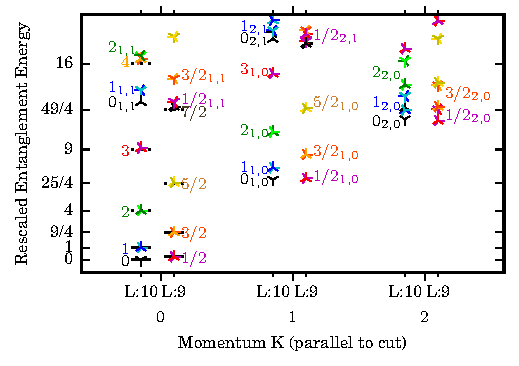
\includegraphics[width=\columnwidth]{EEIdentify.pdf}
	\caption{The identification of the primary states $\ket{\pm e, m=0}$ and the level $n, \bar{n}$ 
	descendants in the spectrum of the soft-core boson entanglement Hamiltonian. The states are labeled 
	$e_{n, \bar{n}}$. The zero and scale of the numerical spectrum are set by matching the lowest two 
	states. The energies and charges of the primaries with charges $2, 5/2, ... 4$ appear at the predicted 
	spots.  The best estimate for the Luttinger parameter from this spectrum is $\kappa \approx 1/6.4$, 
	taken from the energy of the $0_{1, 0}$ state. }
	\label{fig:EEIdentify}
\end{figure}

We can also take the lowest-lying Schmidt state, interpret it as the 
ground state of a 1d Hamiltonian, and consider its entanglement.

\begin{figure}[htbc]
	\centering
	\includegraphics[width=\columnwidth]{{EdgeGS_EntanglementEntropy.pdf}}
	\caption{Entanglement entropy within the entanglement ground state 
of the soft-core boson state on $10$ sites. For comparison, the 
Cardy-Calabrese formula $S(x) = c/3 \log \sin( \pi x/L) + const.$ is 
shown with $c=\frac{1}{2}, 1,$ and $2$, with the $const.$ fixed by 
matching the maximum of the entanglement entropy data. $c=1$ is a good 
fit.}
	\label{fig:EdgeGS_EE}
\end{figure}

\subsection{Symmetry action on the edge}
\label{sec:symmetry}

Gapless entanglement spectra have been shown to be robust features of
 two-dimensional topological and symmetry protected topological (SPT) 
 phases. \brayden{Ref needed}. Combined with the vanishing of 
 topological entanglement entropy, these spectra suggest that the 
 featureless bosonic insulator state \ref{eq:def} is in a SPT phase 
 for some protecting symmetry group $G$. By studying the action of the 
 symmetries of the wavefunction on the  entanglement edge, we can  
 figure out which group $G$, if any, protects it, and find a  
 topological invariant that detects wavefunctions in that phase.
 
%If this is the case, the entanglement edge, and any physical edge respecting the symmetries in $G$, will be degenerate throughout the phase, either via gapless or spontaneous symmetry breaking behavior. If we had a parent Hamiltonian for a state in this phase, the entanglement behavior would be robust to pertubations of that Hamiltonian that respect $G$.

We expect to need lattice symmetries in the protecting group $G$. 
Without lattice symmetries, the state could be adiabatically connected 
to a product state with one boson on each site in the A sublattice. 
Since the topological invariants for interacting states with lattice 
symmetries in more than one dimension aren't well understood, we'll 
first study the symmetry properties using tools designed for 1D 
states, in the same quasi-1D cylindrical geometry we have used above.

For an injective MPS, the action of the symmetries of the wavefunction 
can be determined uniquely on the virtual legs of the MPS. 
\cite{pollmann2010}.


\begin{figure}[htbc]
    \centering
    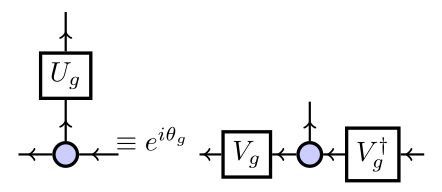
\includegraphics[width=0.6\columnwidth]{group_sym.png}
    \label{fig:mps_group_sym}
\end{figure}

\begin{figure}[htbc]
    \centering
    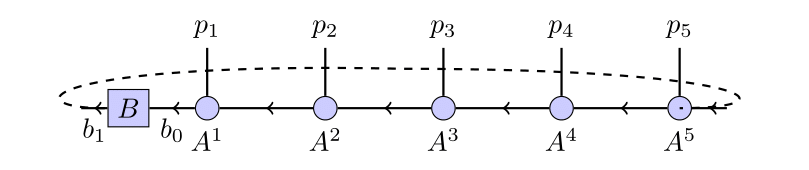
\includegraphics[width=\columnwidth]{mpsbc.png}
    \label{fig:mps_boundary}
\end{figure}

\begin{tabular*}{\columnwidth}{@{\extracolsep{\stretch{1}}}*{5}{r}@{}}
\toprule
$\mathbf{G}$ & $\mathbf{U_g}$ & $\mathbf{\theta_g}$ & $\mathbf{V_g}$ &$\mathbf{V_g V^*_g}$ \\
\midrule
 $U(1) $ & & & & \\
 $\mathcal{\pi} \mathcal{I}_x$ & & & & \\
 $\mathcal{I}_x \mathcal{I}_y$ & & & & \\
 $\mathcal{\pi} \mathcal{I}_x \mathcal{I}_y$ & & & & \\
\bottomrule
\end{tabular*}

Since 
$$  
V_{\mathcal{\pi} \mathcal{I}} V_{\mathcal{\pi} \mathcal{I}}^* = -I \text{\quad or \quad } V_{\mathcal{\pi}} V_{\mathcal{I}} = - V_{\mathcal{I}} V_{\mathcal{\pi}},
$$ 

the representation is in the nontrivial class of 

$$
H^2(\mathbb{Z}_2 \times \mathbb{Z}_2^{\mathcal{I}}; U(1)) = \mathbb{Z}_2.
$$